\section{Mini-WebVision transfer across three bases}
\label{sec:minipilot}
The fixed recipe was transferred to the first 50 original classes of WebVision1.0,
using 65,944 Google training images and 2,500 official validation images for final
evaluation. A fixed noisy split reserves 6,594 training images for checkpoint and
policy selection; the remaining 59,350 supply training trajectories. Three
independent base initializations 42/43/44 each use three nested head seeds.
All 50 epochs completed; noisy-validation CE selected epochs 2/3/3 respectively.
The dataset realization, split and scientific configuration agree across bases.

All bases required recovery after memory-related interruption: base 42 resumed
after 40 epochs, with loader workers reduced from 4 to 0; bases 43/44 used workers 0
throughout and resumed after 43 epochs. Saved optimizer, RNG and target/history
state were restored. The corresponding history prefixes match exactly; a
bit-identical counterfactual uninterrupted run is not asserted.

\begin{table}[t]
\centering
\begin{tabular}{lrrrrr}
\toprule
Method & Base42 & Base43 & Base44 & Mean & Error AUROC \\
\midrule
FP32 base & 83.48 & 82.92 & 82.32 & 82.91 & 0.8853 \\
Uniform TTA & 83.24 & 83.32 & 83.44 & 83.33 & 0.8853 \\
Static & 83.32 & 83.47 & 83.48 & 83.42 & 0.8662 \\
Augmented static & 83.27 & 83.41 & 83.49 & 83.39 & 0.8645 \\
History-50 & 83.65 & 83.92 & 83.79 & 83.79 & 0.7541 \\
Early-5 & 84.13 & 83.83 & 84.29 & 84.08 & 0.8897 \\
\bottomrule
\end{tabular}

\caption{Mini-WebVision accuracy (\%) across independent bases. Learned methods
average three nested heads per base, then bases equally. They are not ensembles.
Error AUROC is the equally weighted mean for original-view FP32 base errors.
Each method uses its own noisy-validation policy.}
\label{tab:minipilot}
\end{table}

Early-5 accuracies are 84.13/83.83/84.29\%, compared with selected uniform
TTA 83.24/83.32/83.44\% and augmented-static 83.27/83.41/83.49\%.
Mean gains over TTA and the augmentation control are 0.75 and 0.69 percentage
points, positive on every base. The between-base sample SD of gains over TTA
is 0.21 points, not a confidence interval. Only three of nine nominal conditional
per-head accuracy intervals strictly exclude zero for each comparison; three
touch zero against TTA and two touch zero against the augmentation control.
These nine heads span only three independent bases and share the evaluation set.

History-50 obtains 83.65/83.92/83.79\% accuracy. Early-5 gains 0.48/-0.09/0.51 points,
averaging 0.30 points; only two of nine conditional accuracy intervals are strictly
positive. Early-5 therefore does not dominate full-history averaging on every
base. Mean original-view error AUROC is 0.8897 versus MSP 0.8853 and History-50
0.7541; the Early-5 mean exceeds MSP on each base, but no paired significance
claim against MSP follows from these point estimates. All nine nominal paired
AUROC intervals against History-50 and augmented-static are positive.

Mean Early-5 ECE/NLL are 0.0195/0.5803, compared with TTA 0.0205/0.5849.
NLL improves over selected TTA on all three bases; ECE worsens on bases 43/44
despite its lower three-base mean. History-50 has lower mean ECE (0.0171).
Accuracy, error ranking and calibration therefore require separate interpretation.

\begin{figure}[t]
\centering
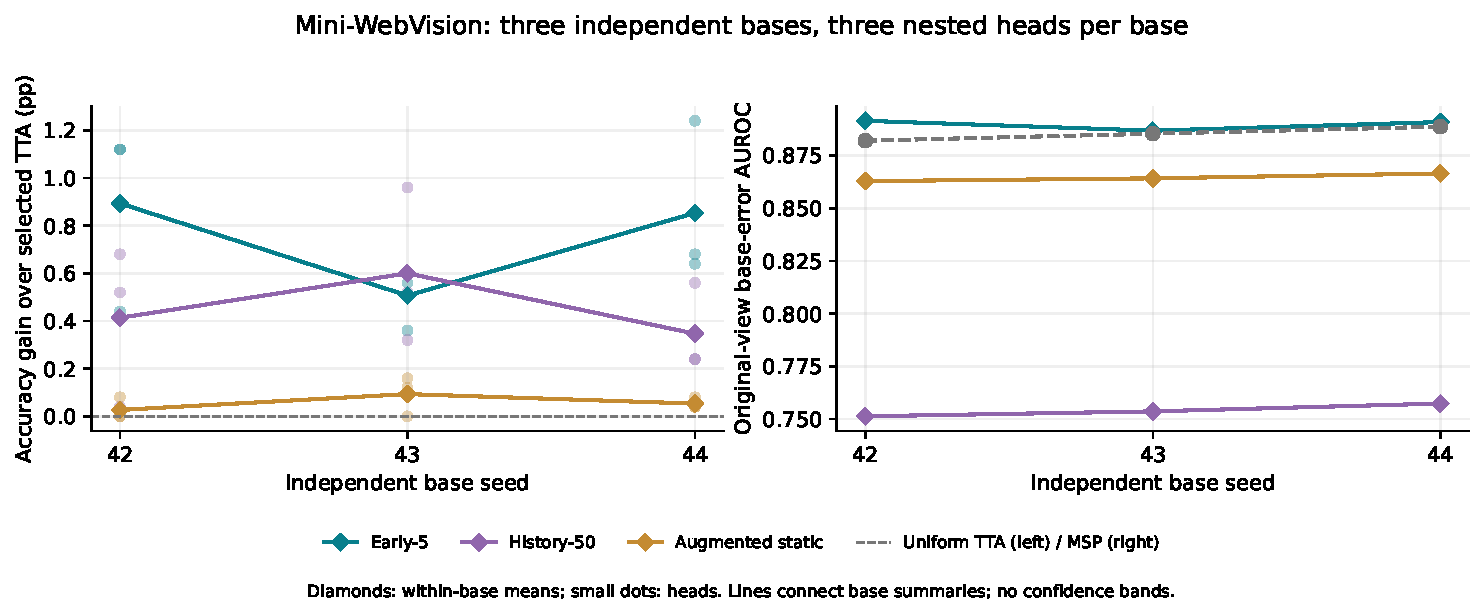
\includegraphics[width=\linewidth]{figures/miniwebvision_replications.pdf}
\caption{Mini-WebVision: within-base means across three independent initializations.
Small dots show nested head gains; connecting lines are not confidence bands.}
\label{fig:minipilot}
\end{figure}

The resumed pipelines took 2.32/2.04/1.96 hours, excluding image preparation and
all earlier interrupted work. Training-stage AMP base accuracies are
83.44/82.88/82.32\%; downstream comparisons consistently use the separately
recorded FP32 values83.48/82.92/82.32\%. Saved compact tables, policy choices
and checkpoint digests agree, but raw-prediction replay remains unperformed.
ImageNet pretraining overlaps the benchmark category space, so this is neither
unseen-category transfer nor a directly comparable state-of-the-art claim.
